%%%%%%%%%%%%%%%%%%%%%%%%%%%%%%%%%%%%%%%%%%
% INITALIZATION AND PACKAGES
%%%%%%%%%%%%%%%%%%%%%%%%%%%%%%%%%%%%%%%%%%

\documentclass[11pt]{article}

\usepackage{geometry}                
\geometry{a4paper}                   

\usepackage{graphicx} % Include pictures
\usepackage{amssymb} % Math functions
\usepackage{amsmath} % Math functions
\usepackage{epstopdf}
%\usepackage{natbib}

% load package with ``framed'' and ``numbered'' option.
\usepackage[numbered, autolinebreaks, useliterate]{mcode} % for including MATLAB code


\usepackage[nottoc,numbib]{tocbibind} % Include the references in the table of content

\usepackage[labelfont=bf]{caption} % Put 'figure' of caption in bold

\DeclareGraphicsRule{.tif}{png}{.png}{`convert #1 `dirname #1`/`basename #1 .tif`.png}

\setlength{\parindent}{1cm} % Set an indentation for every paragraph in the document

%\title{Title}
%\author{Name 1, Name 2}
%\date{date} 

%%%%%%%%%%%%%%%%%%%%%%%%%%%%%%%%%%%%%%%%
% START THE DOCUMENT
%%%%%%%%%%%%%%%%%%%%%%%%%%%%%%%%%%%%%%%%

\begin{document}


\thispagestyle{empty}

\begin{center}

\includegraphics[width=5cm]{ETHlogo.eps}

\bigskip
\bigskip
\bigskip


\LARGE{ 	Lecture with Computer Exercises:\\ }
\LARGE{ Modelling and Simulating Social Systems with MATLAB\\}

\bigskip
\bigskip
\bigskip
\bigskip

\small{Project Report}\\

\bigskip
\bigskip
\bigskip


%\begin{tabular}{|c|}
%\hline
%\\
%\textbf{\LARGE{Inter-State Collaboration Following a}}\\
%\textbf{\LARGE{Zombie Outbreak}}\\
\huge{\bf{Zombie Outbreak:\\The Effect of Inter-State Collaboration on the Survival of Humanity}}
%\\
%\hline
%\end{tabular}

\bigskip
\bigskip
\bigskip


\small{by\\}
\bigskip
\bigskip
\LARGE{Matthieu G. \textsc{Mottet}\\Basile I. M. \textsc{Wicky}}

\bigskip
\bigskip
\bigskip
\bigskip
\bigskip
\bigskip
\bigskip
\bigskip
\bigskip
\bigskip
\bigskip
\bigskip
\bigskip
\bigskip
\bigskip
\bigskip
\bigskip
\bigskip
Zurich\\
December 2012\\

\end{center}


 % Load the cover generated separately
\newpage

\section*{Agreement for free-download} % * removes it from the table of content
\thispagestyle{empty} % Remove page number here

\bigskip
\bigskip

\large We hereby agree to make our source code for this project freely available for download from the web pages of the SOMS chair. Furthermore, we assure that all source code is written by ourselves and is not violating any copyright restrictions.

\begin{center}

\bigskip
\bigskip

\begin{tabular}{@{}p{2cm}@{}p{6cm}@{}@{}p{6cm}@{}}
\begin{minipage}{3.3cm}
\end{minipage}
&
\begin{minipage}{6cm}
\vspace{3cm} \large{Matthieu G. \textsc{Mottet}}

\vspace{\baselineskip}

\end{minipage}
&
\begin{minipage}{6cm}

\vspace{3cm}\large{Basile I. M. \textsc{Wicky}}
\vspace{\baselineskip}
\end{minipage}
\end{tabular}


\end{center}
\newpage


\addtocounter{page}{1} % Add an extra page number to allow the merging with the pdf of the declaration of confidentiality

% IMPORTANT
% you MUST include the ETH declaration of originality here; it is available for download on the course website or at http://www.ethz.ch/faculty/exams/plagiarism/index_EN; it can be printed as pdf and should be filled out in handwriting

% TABLE OF CONTENT
\tableofcontents

\newpage


% ABSTRACT 
\section{Abstract}\indent

Investigation of the application of the SIR model to a zombie outbreak has already been studied, raising the fear of dark days for humanity. However, we would like to deepen this investigation to a multi-state system to see how interactions between subpopulation may brighten the future of the human race. Moreover, we are interested in seeing to what extent the different paradigms of international politics, Realpolitik, Liberalism and Neoconservatism as defined by Daniel W. Drezner in Theories of International Politics and zombies may lead to different outcomes.

% INDIVIDUAL CONTRIBUTION
\section{Individual contributions}\indent

M.G.M. and B.I.M.W. formulated the question in mathematical terms and discussed the implementation in MATLAB. M.G.M. wrote the code. M.G.M. and B.I.M.W. analysed and discussed the results and B.I.M.W. wrote the report.

% ACKNOWLEDGMENTS
\section{Acknowledgments}\indent

We wish to thank Karsten Donnay and Stefano Bielleti for there support in our work, fruitful discussions and an open mind to accept such a project. We would also like to thank the chair of sociology for the computational support provided with simulation time on Brutus.

\newpage

% INTRODUCTION AND MOTIVATION
\section{Introduction and Motivations}\indent

While models of international relationship have already been studied under different pressure components, the effect of a zombie outbreak on international collaboration and equilibrium is a question that has been underestimated and was never addressed to the best of our knowledge. It is remarkable that the effect of such an intense event has not been looked at, although the fear of zombies and the threat they represent is vivid for many of us as reflected by the importance of the zombie culture. zombies, compared to other unnatural creatures such as vampires or aliens, have the very peculiar property not to be a minority inside the human civilization but rather to be in a way a part of it, just not quite as it was, i.e. zombified. Accordingly, zombies cause a much more deep-rooted fear as they not only threaten our lifes but also the our sense of identity as it questions our notion of what humanity is. The psychological effect of such a non-standard threat as well as the repercussion on the behaviour of large popluation systems such as states should be far from trivial. Accordingly, we decided to simulate the inter-state collaboration models in order to see the outcome on a large scale of such an extreme event. While some people might question the validity of such a study (no zombie has been observed so far), we think that the applicablity of such a reasoning could extend to a more probable large-scale epidemological event or simply, give a line of reasoning to cope with what former U.S. Secretery of Defense Donald Rumsfeld referred as the "unknown unknowns" of international security. Zombies might not be real, but the threat and stress they could impose on current world politics is. 

% DESCRIPTION OF THE MODEL
\section{Description of the Model}\indent

\begin{figure}[h!]
\centering
%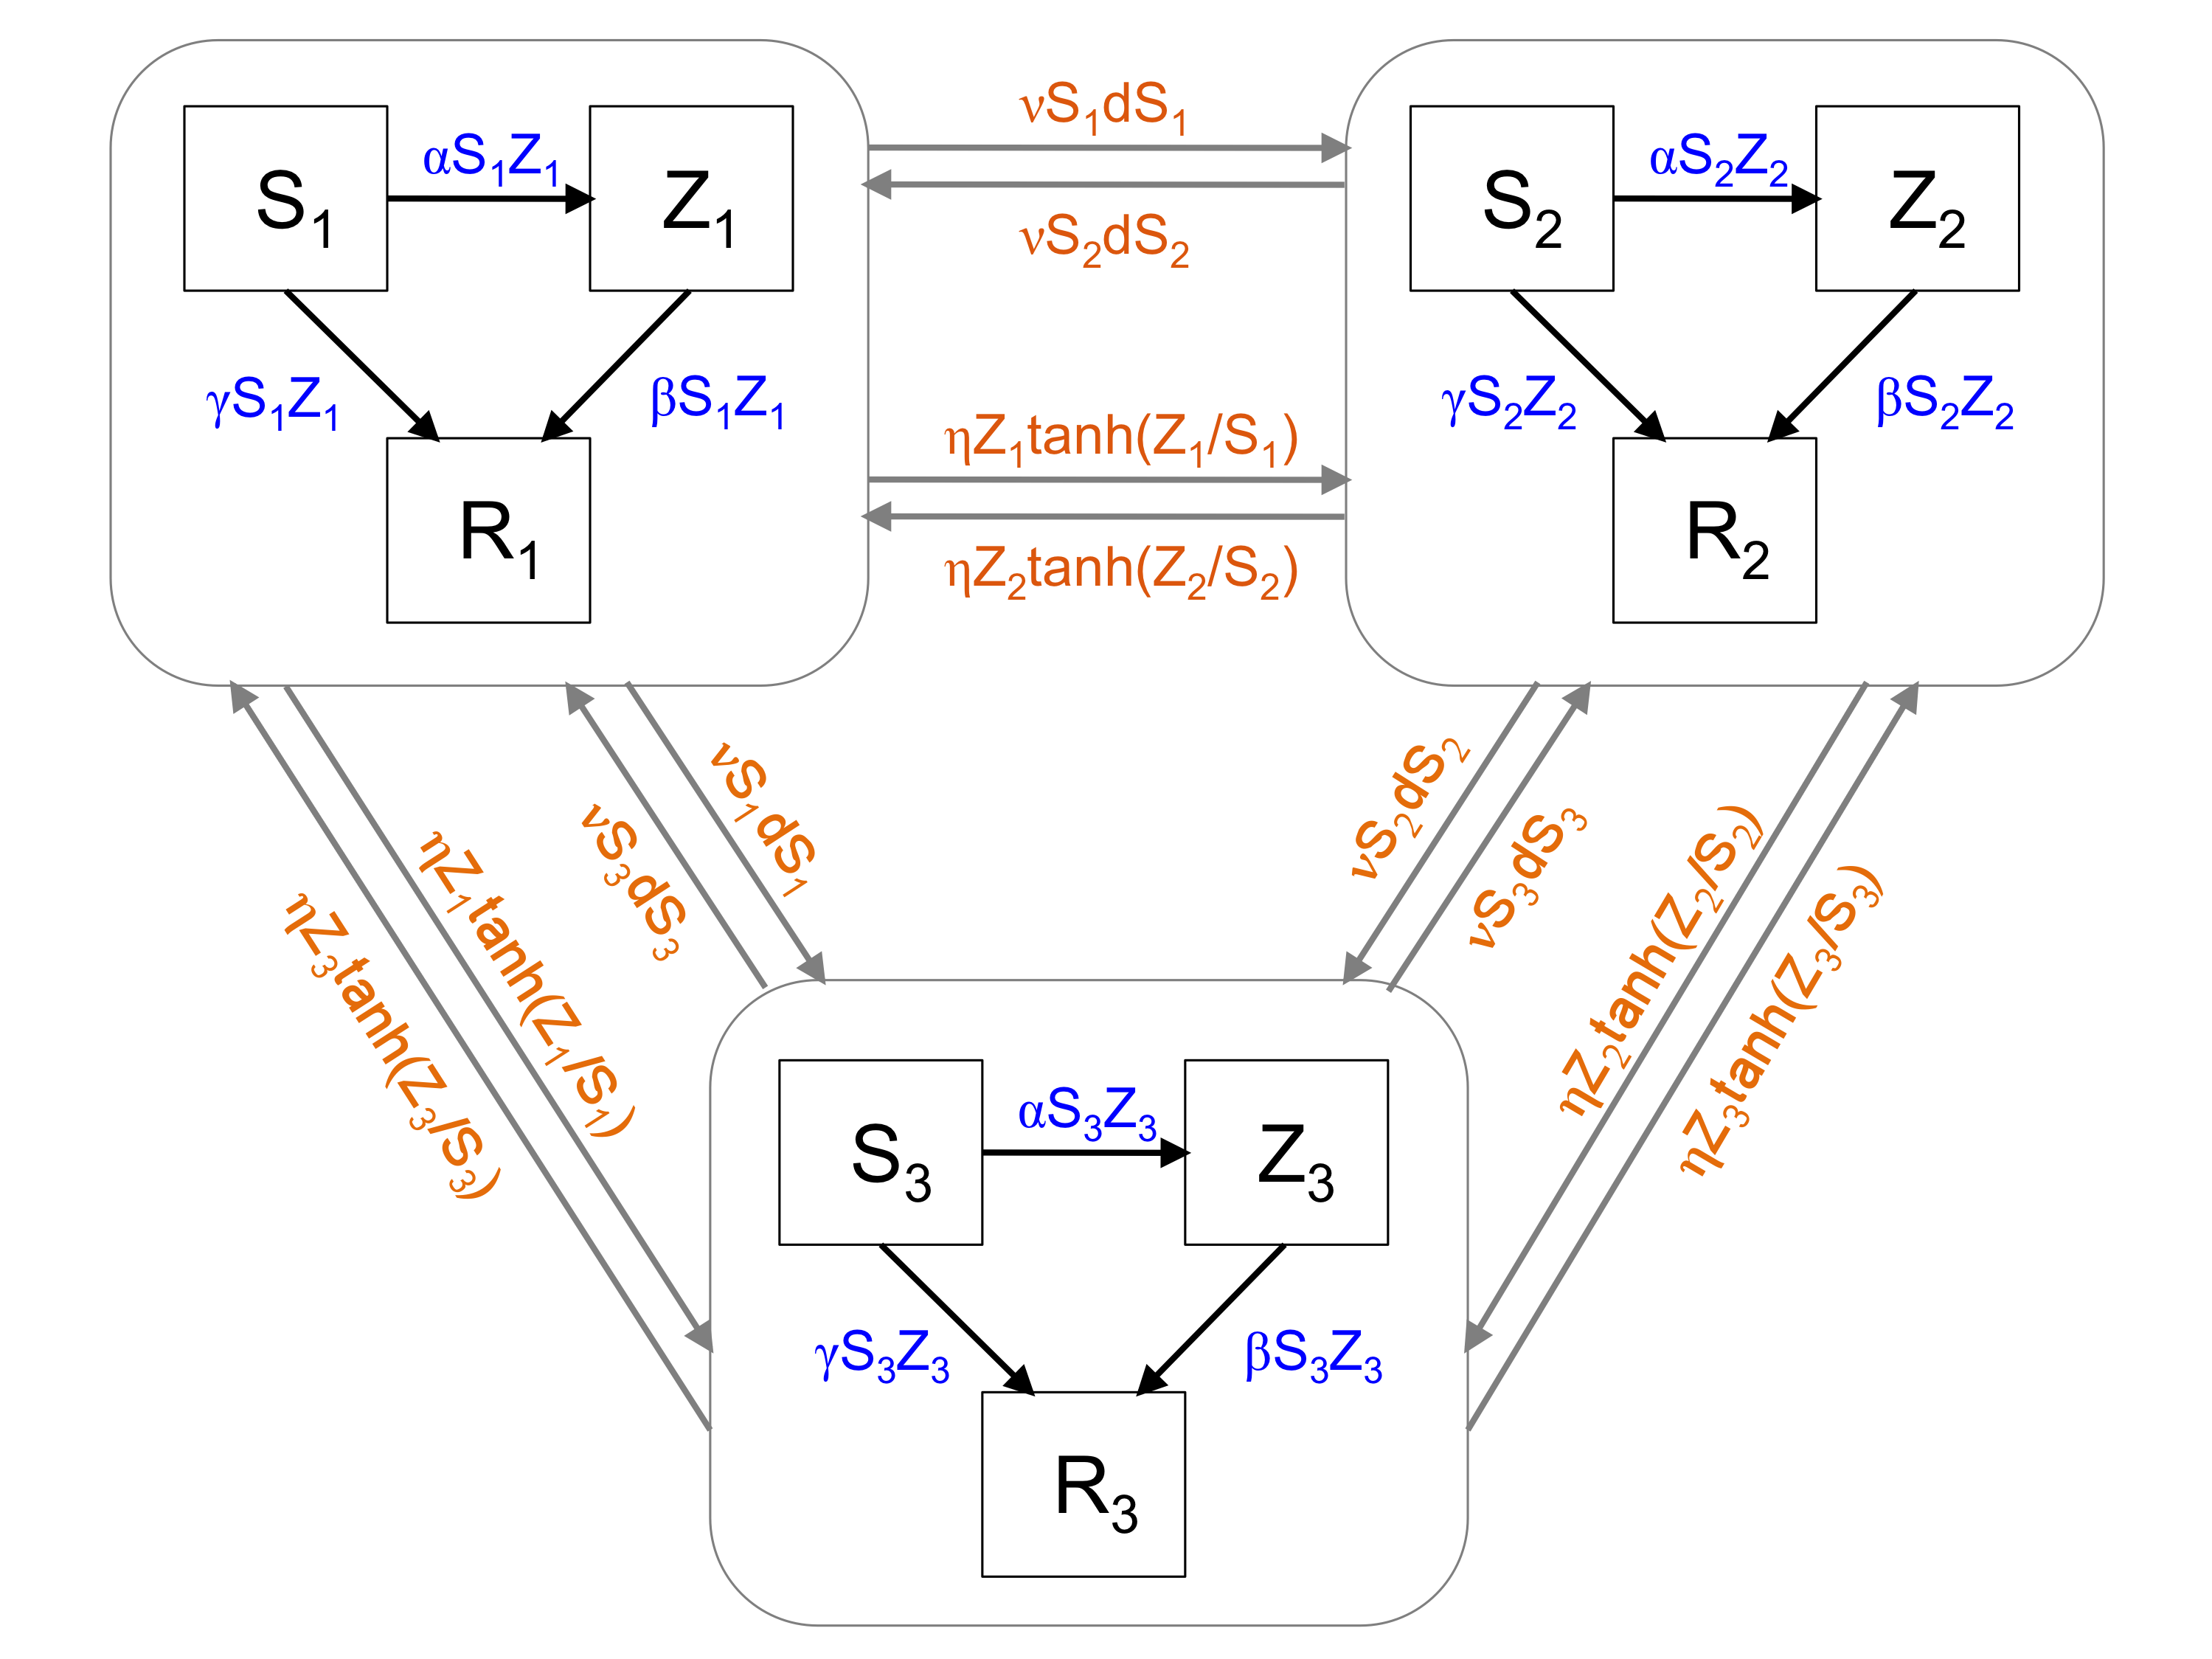
\includegraphics[scale=0.15]{Zombie_model.png}
\caption{Schematic of our model including all variables. The parts in blue represent the fluxes at the micro-state level while the parts in orange represent the macro-state population fluxes. This schematic represent our simulated system where the interaction of three states (micro-states) is modeled }
\end{figure}

\begin{equation}
\Delta S_{i}^{micro} = -\alpha S_{i} Z_{i} -\gamma S_{i} Z_{i} = -(\alpha + \gamma) S_{i} Z_{i}
\end{equation}

\begin{equation}
\Delta Z_{i}^{micro} = +\alpha S_{i} Z_{i} - \beta S_{i} Z_{i} = (\alpha - \beta) S_{i} Z_{i}
\end{equation}

\begin{equation}
\Delta R_{i}^{micro} = +\beta S_{i} Z_{i} + \gamma S_{i} Z_{i} = (\beta + \gamma) S_{i} Z_{i}
\end{equation}

\begin{equation}
\Delta S_{i}^{macro} = -\nu S_{i} \Delta S_{i} + \sum_{j\neq i}{\nu S_{j} \Delta S_{j}}
\end{equation}

\begin{equation}
\Delta Z_{i}^{macro} = -\eta Z_{i}\tanh (\frac{Z_{i}}{S_{i}}) + \sum_{j\neq i}{\eta Z_{j}\tanh (\frac{Z_{j}}{S_{j}})}
\end{equation}

For each state (microstate), we define a SZR model that evaluates the evolution of the different populations under studies: susceptibles (S), zombies (Z) and removed (R). Epidemological-like transfer of populations between the states (at the macrostate level) also occurs as defined above and models the refugees and zombie transfer across states. Those transfers are parameters dependants, which depend on the cost-hypothesis as defined by the Game-Theoretical paradigm implemented. The apparition of zombies in one state will start the game. Each state will then evolve on the domestic and international level. The domestic level will follow a standard SZR model, whereas the international level will introduce exchange in the population of suceptible and zombie between the states. These exchanges will be influenced by the state decisions on foreign policies such as humanitarian or military actions determined by our game theory framework. The Game-Theoretical framework is defined as the possibility of undertaking military action of foreign soil (exporting S) or changing the refugee politics by modifying the mu parameter (allowing more S to come into one's state, and with a collateral cost of having more zombies crossing as well). Each action will be defined with a specific payoff, which in turn will depend on the international cooperation system under scrutiny. For simplicity, we will only model homogenous systems, i.e. all the states will adopt the same international politics paradigm. Finally, we will also introduce a "feedback" loop on the payoff depending on the success of a previously undertaken action (positive or negative affectation of the payoffs). This effect models the psychological effect of a successful or unsuccessful action on future action, for example the effectiveness of a military attack. This effect will be made as to converge after a certain time to model the wearing out of the psychological effect over time. The system will be implemented as a step-based update. This implies the ignorance of the actors (the states) of the action of the other actors. This rationalisation comes as the idea that the outbreak would occur over a short period of time, forcing for rapid decision-making and therefore not allow a reaction-based decision-making process. 

% IMPLEMENTATION
\section{Implementation}\indent
Research Methods

We would like to tackle this question by using a two-level model. Intra-state populations would be modelled by a standard SIR (Kermack-McKendrick) model or an evolution of it that might include quarantined poplutions and more evolved parameters. On the next level, the inter-state relationships would be modelled using Game-Theory under different cost-hypothesis related to the main paradigms of international relationships as previously defined.
Other

The material necessary for defining our models of zombies and 'zombification' parameters will be extracted from the canon of the zombie popular culture such as World War Z (Brooks, 2006), 28 Days Later (Boyle, 2002), The Night of the Living Dead (Romero, 1968), Zombieland (Fleischer, 2009), Resident Evil (Capcom, 1996), etc.

% SIMULATION RESULTS AND DISCUSSION
\section{Simulation Results and Discussion}\indent
Fundamental Questions

Investigation of the application of the SIR model to a zombie outbreak has already been studied, raising the fear of dark days for humanity. However, we would like to deepen this investigation to a multi-state system to see how interactions between subpopulation may brighten the future of the human race. Moreover, we are interested in seeing to what extent the different paradigms of international politics, Realpolitik, Liberalism and Neoconservatism as defined by Daniel W. Drezner in Theories of International Politics and zombies may lead to different outcomes.
Expected Results

As describe in Drezner's book, we except different equilibrium outcomes depending on the paradigm under consideration. He postulates the possibile appearance of zombie states under Realpolitik and Liberalism paradigms while Neoconservatism would not allow such an outcome.

% SUMMARY AND OUTLOOK
\section{Summary and Outlook}\indent

blablabla\cite{reluga2009sis}

% REFERENCES

\bibliography{zombie_report} % Load the .bib file containing the references
\bibliographystyle{unsrt} % Define bibliography style
\nocite{bennett1995modelling, balcan2011phase, funk2010modelling, reluga2010game, reluga2009sis, munz2009zombies, drezner2011theories}

\section{Appendix}

\subsection{outbreak.m}
\lstinputlisting{/Users/basilewicky/zombie_outbreak/code/outbreak.m}
\bigskip
\bigskip
\bigskip

\subsection{update.m}
\lstinputlisting{/Users/basilewicky/zombie_outbreak/code/update.m}
\bigskip
\bigskip
\bigskip

\subsection{plotResults.m}
\lstinputlisting{/Users/basilewicky/zombie_outbreak/code/plotResults.m}
\bigskip
\bigskip
\bigskip




\end{document}  



 
